\documentclass{scrartcl}
\usepackage[parfill]{parskip}
\usepackage{graphicx}
\usepackage{amssymb}
\usepackage{amsmath}
\DeclareMathOperator*{\argmax}{arg\,max}
\DeclareMathOperator*{\argmin}{arg\,min}
\usepackage{url}
\usepackage{hyperref}

\newcommand{\norm}[1]{\left\lVert#1\right\rVert}

\begin{document}

\title{Unpaired Image-to-Image Translation
using Cycle-Consistent Adversarial Networks}
\author{Sebastian Rietsch}

\maketitle
\begin{abstract}
Approach for learning to translate an image from a source domain $X$ to a target domain $Y$ in the absence of paired examples. The goal is to learn a mapping $G: X \rightarrow Y$ such that the distribution of images from $G(X)$ is indistinguishable from the distribution of $Y$ using adversarial loss. Because the mapping is highly under-constrained it gets coupled with an inverse mapping $F: Y \rightarrow X$ and an cycle consistent loss gets introduced to enforce $F(G(X)) \approx X$.
\end{abstract}

\section*{Introduction}
Given: one set of images from domain $X$ and a different set from domain $Y$. One way to achieve this goal is to train a mapping $G: X \rightarrow Y$ such that the output $\hat{y} = G(x), x \in X$, is indistinguishable from images $y \in Y$ by an adversary trained to classify $\hat{y}$ apart from $y$. The optimal $G$ thereby translates the domain $X$ to a domain $\hat{Y}$ distributed identically to $Y$. However, such a translation does not guarantee that an individual input $x$ and output $y$ are paired up in a meaningful way - there are infinitely many mappings $G$ that will induce the same distribution over $\hat{y}$. Also: it is really hard to optimize such an adversarial objective (mode collapse).

These issues call for adding more structure to our objective. Translations should be cycle-consistent, in the sense that if we translate e.g. a sentence from English to French, and then translate it back from French to English, we should arrive back at the original sentence. Mathematically: two translators $G: X \rightarrow Y$ and $F: Y \rightarrow X$, $G$ and $F$ should be inverse of each other and both should be bijections.

This structural assumptions gets applied by training both mappings $G$ and $F$ simultaneously and adding a \textit{cycle consistency loss} that encourages $F(G(x)) \approx x$ and $G(F(y)) \approx y$. Combining this loss with adversarial losses on domain $X$ and $Y$ yields the full objective for unpaired image-to-image translation.

\section*{Formulation}
The goal is to learn mapping functions between two domains $X$ and $Y$ given training examples $\{x_i\}_{i=1}^N$ where $x_i \in X$ and $\{y_j\}_{j=1}^M$ where $y_j \in Y$. We denote the data distribution as $x \sim p_{data}(x)$ and $y \sim p_{data}(y)$. The model includes two mappings $G: X \rightarrow Y$ and $F: Y \rightarrow X$. In addition, two adversarial discriminators $D_X$ and $D_Y$ get introduced, where $D_X$ aims to distinguish between images $\{x\}$ and translated images $\{F(y)\}$; in the same way, $D_Y$ aims to discriminate between $\{y\}$ and $\{G(x)\}$. the objective contains two types of terms: adversarial losses for matching the distribution of generated images to the data distribution in the target domain; and cycle consistency losses to prevent the learned mapping $G$ and $F$ from contradicting each other.

\subsection*{Adversarial Loss}
For the mapping function $G: X \rightarrow Y$ and its discriminator $D_Y$, the loss is:
\begin{equation}
\begin{split}
\mathcal{L}_{GAN}(G, D_Y, X, Y) &= \mathbb{E}_{y \sim p_{data}(y)} [log(D_Y(y))]\\
 &+ \mathbb{E}_{x \sim p_{data}(x)}[log(1 - D_Y(G(x))],
\end{split}
\end{equation}
where $G$ tires to generate images $G(x)$ that look similar to images from domain $Y$, while $D_Y$ aims to distinguish between translated samples $G(x)$ and real samples $y$. $G$ aims to minimize this objective against an adversary $D$ that tries to maximize it, i.e. $min_G max_{D_Y} \mathcal{L}_{GAN}(G, D_Y, X, Y)$. A similar adversarial loss for the mapping function $F: Y \rightarrow X$ and its discriminator $D_X$ gets introduced as well: i.e. $min_F max_{D_X} \mathcal{L}_{GAN} (F, D_X, Y, X)$.

\subsection*{Cycle Consistency Loss}
As already discussed, adversarial loss alone cannot guarantee that the learned function can map an individual input $x_i$ to a desired output $y_i$. To further reduce the space of possible mapping functions, we argue that the learned mapping functions should be cycle-consistent. Two types:
\begin{itemize}
	\item
		The image translation cycle should be able to bring $x$ back to the original image, i.e. $x \rightarrow G(x) \rightarrow F(G(x)) \approx x.$ We call this \textit{forward cycle}.
	\item
		For each image $y$ from domain $Y$, $G$ and $F$ should also satisfy \textit{backward cycle consistency}: $y \rightarrow F(y) \rightarrow G(F(y)) \approx y$.
\end{itemize}
From this follows the \textit{cycle consistency loss}:
\begin{equation}
\begin{split}
\mathcal{L}_{cyc}(G, F) &= \mathbb{E}_{x \sim p_{data}(x)}[\norm{F(G(x)) - x}_1] \\
& + \mathbb{E}_{y \sim p_{data}(y)}[\norm{F(G(y)) - y}_1]
\end{split}
\end{equation}
Replacing the L1 norm in this loss with an adversarial loss between $F(G(x))$ and $x$ and vice verse did not induce improved performance.

\begin{figure}
	\centering
		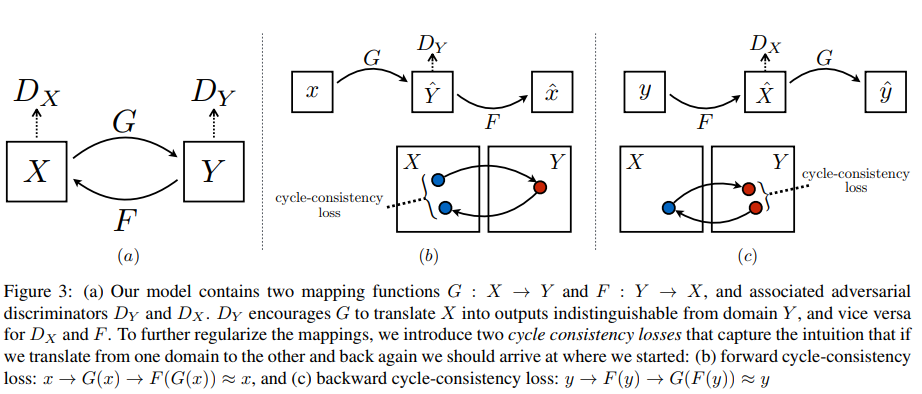
\includegraphics[scale=0.6]{cyclegan}
	\label{fig:cyclegan}
\end{figure}

\subsection*{Full objective}
The full objective is
\begin{equation}
\begin{split}
	\mathcal{L}(G, F, D_X, D_Y) &= \mathcal{L}_{GAN} (G, D_Y, X, Y)\\
	&+ \mathcal{L}_{GAN}(F, D_X, Y, X)\\
	&+ \lambda \mathcal{L}_{cyc} (G, F),
\end{split}
\end{equation}
where $\lambda$ controls the relative importance of the two objectives. We aim to solve:
\begin{equation}
	G^*, F^* = argmin_{G, F} max _{D_X, D_Y} \mathcal{L}(G, F, D_X, D_Y)
\end{equation}
The model can be viewed as training two autoencoders: we learn on autoencoder $ F \circ G: X \rightarrow X$ jointly with another $ G \circ F: Y \rightarrow Y$. These autoencoders each have special internal structured: they map an image to itself via an intermediate representation that is a translation of the image into another domain. 

\section*{Implementation}
\subsection*{Network Architecture}
\begin{itemize}
	\item
		Generator: Adopted from Johnson et al. \cite{DBLP:journals/corr/JohnsonAL16}
		\begin{itemize}
			\item
				Two stride-2 convolutions, several residual blocks and two fractionally-strided convolutions with stride $\frac{1}{2}$
			\item
				6 blocks for $128 \times 128$ images and 9 blocks for $256 \times 256$ and higher-resolution training images
			\item
				Similar to Johnson et al. instance normalization gets used
		\end{itemize}
	\item
		Discriminator: $70 \times 70$ PatchGANs \cite{DBLP:journals/corr/LiW16b} which aim to classify whether $70 \times 70$ overlapping image patches are real or fake. Such a patch-level discriminator architecture has fewer parameters than a full-image discriminator and can work on arbitrarily-sized images in a fully convolutional fashion
\end{itemize}

\subsection*{Training details}
\begin{itemize}
	\item
		$\mathcal{L}_{GAN}$: replace negative log likelihood objective by a least squares loss \cite{DBLP:journals/corr/MaoLXLW16}. This loss is more stable during training and generates higher quality results. In particular, for GAN loss we train $G$ to minimize $\mathbb{E}_{x \sim p_{data}(x)} [(D(G(X)) - 1)^2]$ and train the $D$ to minimize $\mathbb{E}_{y \sim p_{data}(y)}[(D(y) - 1)^2] + \mathbb{E}_{x \sim p_{data}(x)}[D(G(x))^2]$
	\item
		To reduce model oscillation Shrivastava et al.'s \cite{DBLP:journals/corr/ShrivastavaPTSW16} strategy gets applied, where the discriminator gets updated using a history of generated images rather than the ones produced by the latest generators. An image buffer that stores the 50 previously created images gets kept.
	\item
		$\lambda = 10$ 
	\item
		Adam solver with a batch size of $1$, learning rate of $0.0002$. Same learning rate for the first 100 epochs and linearly decay the rate to zero over the next 100 epochs.
\end{itemize}
\newpage
\bibliographystyle{abbrv}
\bibliography{unpaired_image_to_image_cycleGAN}
\end{document}